\documentclass[a4paper,12pt]{article}
\usepackage[a4paper]{geometry}
\usepackage{polski}
\usepackage[polish]{babel}
\usepackage[utf8]{inputenc}
\usepackage{indentfirst}
\usepackage{graphicx}
\usepackage{lastpage}
\usepackage{fancyhdr}
\usepackage{hyperref}
\usepackage{float}
\usepackage{subfig}
\usepackage{enumitem}
%head & foot
\pagestyle{fancy}
\title{Specyfikacja funkcjonalna projektu \textit{Wireworld} w~języku Java}
\author{Chabik Jan (291060), Łuczak Mateusz (291088)}
\date{26 kwietnia 2018}
\setlength\parindent{24pt}
\setlength{\headheight}{16pt}
\lhead{}
\rhead{Specyfikacja funkcjonalna projektu \textit{Wireworld} w języku Java}
\rfoot{str. \thepage/\pageref{LastPage}}
\cfoot{}

\begin{document}
\maketitle
\thispagestyle{empty}
\begin{center}
	
\includegraphics[scale=0.1]{logo_ee_big.png}
\end{center}
\newpage

\tableofcontents
\pagenumbering{arabic}
\newpage

\section{Opis ogólny}
\subsection{Nazwa programu}
Program został nazwany \texttt{Wireworld}. Nazwa nawiązuje do rozwiązywanego problemu, którym jest stworzenie emulatora \textit{Wireworld} Briana Silvermana.

\subsection{Poruszany problem}
Poruszanym problemem będzie stworzenie emulatora \textit{Wireworld} Briana Silvermana w języku Java.

\textit{Wireworld} jest typem automatu komórkowego zaproponowanym przez Briana Silvermana w roku 1987. Jest to system często używany do symulacji elementów elektronicznych operujących na wartościach bitowo. Pomimo tego, iż sam sposób działania nie jest skomplikowany, jest możliwe zbudowanie funkcjonującego komputera.

Mapa dla danego automatu komórkowego reprezentowana jest przez cztery stany:
\begin{itemize}
\item Komórka pusta;
\item Głowa elektronu;
\item Ogon elektronu;
\item Przewodnik.
\end{itemize}
Komórki są innego koloru, aby rozróżnić każdy ze stanów (przykładowo komórka pusta może być czarna, głowa elektronu niebieska, ogon czerwony, a przewodnik żółty). W jednostce czasowej, każdej komórce przypisywany jest stan na podstawie stanów jej sąsiadów. Rozwiązaniem będzie wizualizacja działającego automatu komórkowego oraz pliki wynikowe opisujące stan automatu.

\subsection{Cel projektu}
Celem projektu jest zapoznanie się przez studentów z problemem \textit{Wireworld} Briana Silvermana oraz stworzenie implementacji w języku Java. Zadanie przewidziane zostało dla grup dwuosobowych. Ze względu na to, ważna jest umiejętność pracy w zespole.

\section{Opis funkcjonalności}
\subsection{Korzystanie z programu}
Program po uruchomieniu zostanie wywołany jako aplikacja okienkowa. \linebreak Wszystkie opcje dostosowania symulacji będą dostępne w środowisku graficznym.

\subsection{Uruchomienie programu}
Uruchomienie programu następuje poprzez aktywację pliku wynikowego w~środowisku IntelliJ Idea.

\subsection{Możliwości programu}
\begin{itemize}
\item Emulacja \textit{Wireworld} Briana Silvermana;
\item Odczyt danych z pliku tekstowego zawierającego informacje dotyczące mapy automatu komórkowego;
\item Generowanie wybranej przez użytkownika ilości generacji automatu komórkowego;
\item Symulacja automatu dla wybranego przez użytkownika sąsiedztwa (wybór spośród sąsiedztwa Moore'a i von Neumanna);
\item Zapis danych wyjściowych do pliku tekstowego oraz pliku \texttt{.png};
\item Możliwość wybrania symulacji automatu w wybranych przez użytkownikach interwałach (np. $\frac{1}{4}s$) oraz pominięcia wybranej ilości generacji.
\end{itemize}

\section{Format danych i struktura plików}
\subsection{Słownik pojęć}
\begin{itemize}
\item \textbf{Plasza} - jest to prostokąt podzielony na pola (komórki), z których każda ma przypisaną wartość (0, 1, 2, 3) oraz odpowiedni kolor (czarny, niebieski, czerwony, żółty). Gdy komórka znajduje się stanie `0' mówimy, że jest pusta. W przypadku stanu `1', jest to głowa elektronu. Stanowi `2' przypisany jest ogon elektronu, a `3' przewodnik;
\item \textbf{Sąsiedztwo Moore'a} - typ sąsiedztwa polegający na tym, iż rozpatrywane są wszystkie 8 komórek sąsiadujących z daną komórką (komórka na północ, południe, wschód, zachód, północny-wschód, północny-zachód, południowy-zachód, południowy-wschód);
\begin{figure}[H]
	\centering
	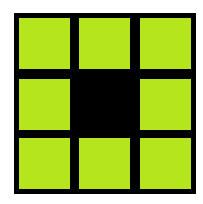
\includegraphics[scale=1]{moore.png}
	\caption{Sąsiedztwo Moore'a. Po środku znajduje się komórka (czarna), dla której rozpatrujemy sąsiadów. Komórki zielone opisują, które z nich są sąsiadami w opisywanym sąsiedztwie.}
\end{figure}
\item \textbf{Sąsiedztwo Von Neumanna} - typ sąsiedztwa polegający na tym, iż rozpatrywane są 4 komórki sąsiadujące (komórka na północ, południe, wschód i zachód);
\begin{figure}[H]
	\centering
	
\includegraphics[scale=1]{von_neumann.png}
	\caption{Sąsiedztwo von Neumanna. Po środku znajduje się komórka (czarna), dla której rozpatrujemy sąsiadów. Komórki zielone opisują, które z nich są sąsiadami w opisywanym sąsiedztwie.}
\end{figure}
\end{itemize}
\subsection{Struktura katalogów}
\begin{figure}[H]
	\centering
	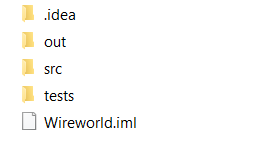
\includegraphics{CatalogueStruct.png}
	\caption{Struktura katalogów projektu}
\end{figure}
Struktura katalogów w projekcie będzie niemalże identyczna ze strukturą projektu stworzonego w IntelliJ Idea. Jedyną różnicą będzie dodatkowy katalog \texttt{tests}, w którym znajdować się będą klasy z testami jednostkowymi dla poszczególnych klas.


\subsection{Przechowywanie danych w programie}
\begin{itemize}
\item Informacje o opcjach zapisane będą w klasie statycznej;
\item Każda macierz zapisana będzie w obiekcie Matrix;
\item Obiekty Matrix trzymane będą w klasie głównej Main.
\end{itemize}

\subsection{Dane wejściowe}
Jako dane wejściowe służy plik w formacie \texttt{.txt}, w którym zapisana jest plansza.

Plik rozpoczyna się wymiarami planszy zapisanej za pomocą liczb naturalnych większych od 0. Następnie podawane są cyfry `0', `1', `2', `3' oznaczające stan komórki (pusta, głowa, ogon, przewodnik). Ilość cyfr powinna odpowiadać wielkości planszy. Przykładowo, jeżeli wymiary macierzy to \texttt{3x4}, to powinno być podanych 12 cyfr oznaczających stan komórek.

\subsection{Dane wyjściowe}
\begin{itemize}
\item Pliki \texttt{.png}, w których znajduje się graficzna interpretacja każdej kolejnej generacji;
\item Pliki w formacie \texttt{.txt}, w których zapisane są kolejne generacje;
\item Zwizualizowana generacja automatu w środowisku graficznym.
\end{itemize}

\section{Scenariusz działania programu}
\subsection{Scenariusz ogólny}
\begin{enumerate}
\item Uruchomienie programu;
\item Wybór pliku wejściowego przez użytkownika;
\item Wybór katalogu wyjściowego przez użytkownika;
\item Załadowanie pliku wejściowego;
\item Opcjonalnie dostosowanie przez użytkownika opcji tworzenia generacji;
\item Uruchomienie automatu;
\end{enumerate}

\subsection{Scenariusz szczegółowy}
\begin{enumerate}
\item Uruchomienie programu:
	\begin{itemize}
	\item Po uruchomieniu programu generuje się okno GUI;
	\item W oknie GUI użytkownik zaznacza następujące opcje:
		\begin{itemize}
			\item Wybór pliku wejściowego;
			\item Wybór katalogu wyjściowego;
			\item Sąsiedztwo;
			\item Ilość generacji;
			\item Zapis do pliku \texttt{.txt} i/lub \texttt{.png}
		\end{itemize}
		Opcje wyboru pliku wejściowego i katalogu wyjściowego są obowiązkowe. Reszta jest wybrana automatycznie, jednakże może być modyfikowana.
	\end{itemize}
\item Wybór pliku wejściowego przez użytkownika:
	\begin{itemize}
		\item Użytkownik za pomocą przycisku pozwalającego na przeszukiwanie katalogów zaznacza plik typu \texttt{.txt}. Program zapisuje ścieżkę do pliku w~postaci zmiennej typu \texttt{String}. W razie braku dostępu do pliku lub sytuacji gdy plik nie jest w formacie \texttt{.txt} wyświetlany jest odpowiedni komunikat.
	\end{itemize}
\item Wybór katalogu wyjściowego przez użytkownika:
	\begin{itemize}
		\item Użytkownik za pomocą przycisku pozwalającego na przeszukiwanie katalogów zaznacza katalog, do którego zapisywane będą pliki \texttt{.txt} i \texttt{.png}. Program zapisuje ścieżkę do katalogu w postaci \texttt{String}. W razie niepoprawnego katalogu wyświetlany jest odpowiedni komunikat 
	\end{itemize}
\item Załadowanie pliku wejściowego:
	\begin{itemize}
	\item Po przyciśnięciu przycisku \texttt{Load File}, program generuje macierz na podstawie pliku wejściowego. Wygenerowaną macierz pokazuje w interfejsie użytkownika. Sprawdzana jest poprawność pliku wejściowego.
	\end{itemize}
\item Opcjonalne dostosowane opcji programu przez użytkownika:
	\begin{itemize}
		\item Za pomocą chechboxów \texttt {TXT} i \texttt {PNG} zaznacza się preferencje co do generowania plików (automatycznie obie opcje są odznaczone);
		\item Za pomocą dropbara \texttt{TimeInterval} wybiera się interwał czasowy \texttt{t}, w~jakim na ekranie mają się pojawiać kolejne generacje (automatycznie wybrana jest 1 sekunda);
		\item Za pomocą radiobuttonów wybiera się sąsiedztwo które ma stosować program (automatycznie wybrane jest sąsiedztwo \texttt {Moore’a});
		\item W okno tekstowe wpisujemy ilość generacji, które program ma wygenerować (automatycznie wpisane jest 5);
	\end{itemize}
\item Uruchamianie automatu
	\begin{enumerate}
	\item Za pomocą przycisku \texttt{One Move}:
		\begin{itemize}
			\item Blokowany jest dostęp do wszystkich przycisków;
			\item Wykonywane jest pojedyncze przejście \textit{(Opis znajduje się w rozdziale 4.3)};
			\item Odblokowywany jest dostęp do wszystkich przycisków.
		\end{itemize}
	\item Za pomocą przycisku oznaczonego zielonym trójkątem (\texttt{START}):
		\begin{itemize}
			\item Blokowany jest dostęp do wszystkich przycisków poza przyciskiem \texttt{STOP};
			\item Włącza się pętla wykonywana n-razy (n to liczba wpisana w pole jako \texttt{NumberOfGenerations});
			\item Każde pojedyncze przejście wykonuje się co \texttt{t} sekund;
			\item Po każdym przejściu sprawdzane jest czy podczas działania programu został naciśnięty przycisk \texttt {STOP}. Jeśli tak, pętla zostaje przerwana i odblokowywany jest dostęp do pozostałych przycisków.
		\end{itemize}
	\end{enumerate}
\end{enumerate}

\subsection{Opis pojedynczego przejścia}
\begin{enumerate}
\item Sprawdzane jest czy w polu \texttt{Number Of Generations} zapisana jest popraw\-na wartość (dodatni \texttt{int} mniejszy od 10 000). W razie błędu na ekranie pojawia się odpowiedni komunikat;
\item Na podstawie opcji, utworzonej macierzy i wartości w polu \texttt{NumberOf \linebreak Generations} program generuje kolejną macierz;
\item Program wyświetla kolejną macierz na pulpicie;
\item Na podstawie opcji program generuje pliki \texttt{.txt} i/lub \texttt{.png};
\item Program odejmuje 1 od wartości wpisanej w pole tekstowe oznaczone jako \texttt{NumberOfGenerations}.
\end{enumerate}

\subsection{Opis środowiska graficznego programu}
\subsubsection{Projekt środowiska graficznego}
\begin{figure}[H]
	\centering
	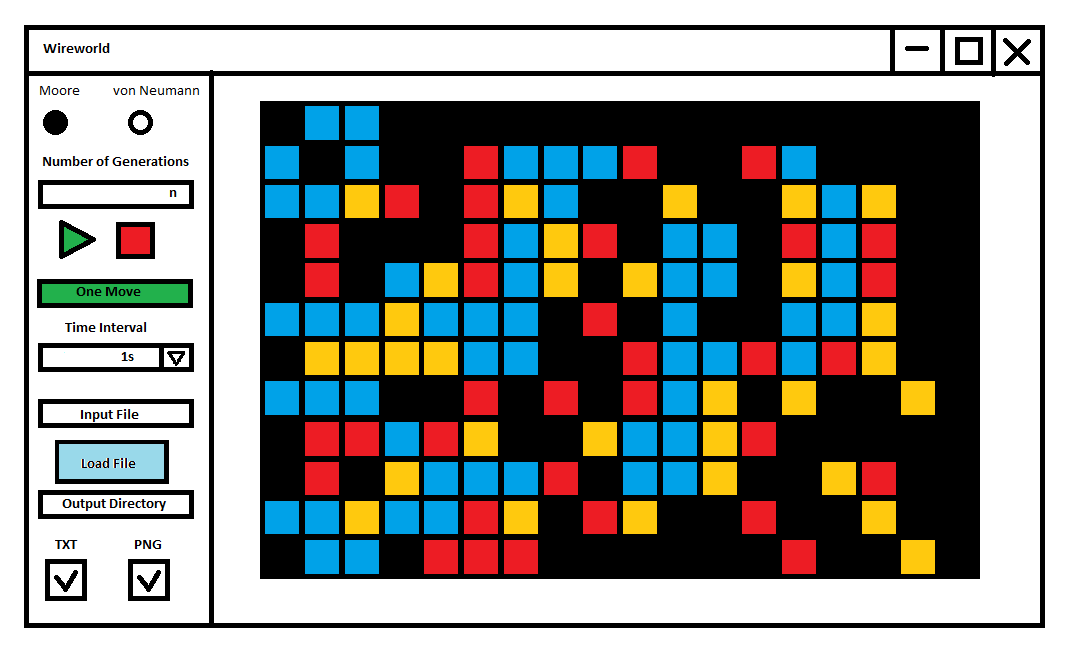
\includegraphics[scale=0.6]{ProjektGUI.png}
	\caption{Projekt środowiska graficznego}
\end{figure}
\newpage
\subsubsection{Opis guzików}
\begin{figure}[H]
	\centering
	\subfloat[Radio Buttons]{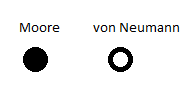
\includegraphics{RadioButtons.png}} \hspace{1cm}
	\subfloat[Number of generations]{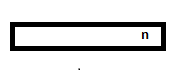
\includegraphics[width=5cm]{NumberOfGenerations.png}}\\
	\subfloat[Start and Stop]{
\includegraphics{StartANDStop.png}} \hspace{1cm}
	\subfloat[One Move]{
\includegraphics{OneMove.png}}\\
	\subfloat[Time Interval]{
\includegraphics{TimeInterval.png}}\hspace{1cm}
	\subfloat[Input File]{
\includegraphics{InputFile.png}} \\
	\subfloat[Load File]{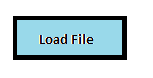
\includegraphics{LoadFile.png}} \hspace{1cm}
	\subfloat[Output Directory]{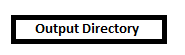
\includegraphics{OutputDirectory.png}} \\
	\subfloat[Save Settings]{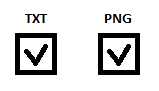
\includegraphics{SaveSettings.png}}
	\caption{Zestawienie wszystkich guzików}
\end{figure}

\begin{enumerate}[label=(\alph*)]
\item Radio Buttons – grupa przycisków pozwalająca wybierać sąsiedztwo;
\item Number of Generations – pole tekstowe, do którego należy wpisać ilość przejść automatu komórkowego (wartość musi być dodatnią liczbą całkowitą mniejszą od 10 000);
\item Start and Stop – przyciski \texttt{START} i \texttt{STOP} pozwalające uruchomić i zatrzymać automat;
\item One Move - przycisk, który sprawia, że automat wykonuje pojedyncze przejście;
\item TimeInterval – przycisk typu Dropbar odpowiadający za interwał czasowy pomiędzy przejściami automatu komórkowego;
\item Input File – przycisk typu FileChooser pozwalający wybrać plik wejściowy;
\item Load File - przycisk z pomocą którego tworzona i wyświetlana w interfejsie jest macierz z pliku wejściowego;
\item Output Directory – przycisk typu FileChooser, za pomocą którego wybieramy katalog, do którego generowane są pliki;
\item Save Settings – 2 przyciski typu CheckBox pozwalające wybierać preferencje dotyczące zapisu generacji.
\end{enumerate}

\section{Testowanie}
Testować działanie programu będziemy za pomocą narzędzi dostępnych w~Frameworku JUnit 4. Dla każdej klasy stworzona zostanie klasa testująca, w której testować będziemy każdą z metod. Skorzystamy z metodyki testów regresywnych, czyli po dodaniu nowej funkcjonalności testować będziemy również poprzednio sprawdzone klasy w celu upewnienia się, czy program działa poprawnie.
\end{document}
